%\subsection{Introduction}\label{introduction}

This section serves as a  introduction to the course of
Blockchains and Decentralized Applications (BDA). It begins by outlining
the course's core objectives, which are designed to provide both
theoretical knowledge and practical skills in this rapidly evolving
domain. 
%The section details the course structure, including the lecture
%schedule, project requirements, and examination policies, to provide a
%clear roadmap for the semester. A significant portion of this
%introduction is dedicated to presenting the instructors, a team of
%seasoned academics and industry practitioners, whose collective
%expertise spans the critical areas of blockchain technology, from
%consensus protocols and system security to zero-knowledge cryptography
%and forensic analysis.

The primary objective of this section is to establish a solid foundation
for the topics that will be explored in subsequent sections. To this
end, it delves into the fundamental cryptographic constructs that are
indispensable for understanding the inner workings of blockchain
systems. These include a detailed examination of cryptographic hash
functions, which ensure data integrity; hash chains, a simple yet
powerful tool for creating cryptographically connected sequences; Merkle trees, an
efficient data structure for verifying the contents of large data sets;
and digital signatures, the mechanism that provides authenticity and
non-repudiation in a decentralized environment. A thorough understanding
of these cryptographic primitives is paramount, as they form the bedrock
upon which the security, immutability, and trustworthiness of
blockchains are built.

\subsection{Learning Objectives of the Course}\label{learning-objectives}

\begin{itemize}
	\tightlist
	\item
	Gain theoretical and practical knowledge in the field of BDA, their
	types, consensual protocols, and pros/cons.
	\item
	Understand the terminology, unique properties of blockchain,
	integrity-preserving data structures, and algorithms.
	\item
	Learn about practical use cases and their potential vulnerabilities.
	\item
	Understand the scalability/throughput problems and their solutions.
	\item
	Grasp the privacy aspects and variants of their solution.
	\item
	Develop the ability to design, implement, and deploy custom DAPPs and
	blockchains.
\end{itemize}

\begin{center}\rule{0.5\linewidth}{0.5pt}\end{center}

\subsection{Course Overview}\label{section-1-course-overview}

\subsubsection{About the Instructors}\label{about-the-instructors}

The course is led by a team of experienced researchers and practitioners
in the field of blockchain technology, each bringing a unique set of
skills and experiences to the curriculum.
The following listings contains current and former course instructors who helped in running this course.
\begin{itemize}
	\item
	\textbf{doc. Ing. Ivan Homoliak, Ph.D.} (Guarantor): Dr.~Homoliak is
	an associate professor at the Faculty of Information Technology, Brno
	University of Technology (FIT@BUT). His academic journey includes a
	Ph.D.~from FIT@BUT in 2016, followed by a postdoctoral fellowship at
	the Singapore University of Technology and Design (SUTD), where his
	research was centered on blockchains and cybersecurity. His
	habilitation, titled ``Towards Secure Consensus Protocols and
	Decentralized Applications in Blockchains,'' \ih{cite} underscores his deep
	expertise in the field. Dr.~Homoliak's research interests are
	extensive and include electronic voting in blockchains~\cite{homoliak2023bbb,venugopalan2023always,stanvcikova2022sbvote,homoliak2025votemate}, the security
	and scalability of consensus protocols~\cite{perevsini2023incentive,perevsini2021dag,perevsini2023dag,budinsky2023fee}, the intersection of Trusted
	Execution Environments (TEE) with blockchain technology~\cite{homoliak2020aquareum}, Central Bank
	Digital Currencies (CBDC)~\cite{homoliak2023cbdc}, and the application of zero-knowledge
	cryptography~\cite{perevsini2025featherwallet} \ih{todo}.
	\item
	\textbf{Ing. Vladimír Veselý, Ph.D.} (Guarantor Deputy): Dr.~Veselý's
	engagement with cryptocurrencies dates back to 2011, when he began
	mining Bitcoin. His practical experience is complemented by a
	Ph.D.~from FIT@BUT. He serves as a consultant for law enforcement
	agencies on cryptocurrency-related crimes, a role that leverages his
	deep understanding of forensic analysis and the tracking of illicit
	activities on the blockchain. His research has involved correlating
	dark market activities with cryptocurrency transactions\ih{cite} and exploring
	the use of blockchains for storing personal named records\ih{cite}.
	\item
	\textbf{Martin Perešíni}: A Ph.D.~student (under supervision of Dr. Homoliak) whose research is
	concentrated on the security and scalability of consensus protocols.
	His work includes the study of Directed Acyclic Graph (DAG) based
	protocols~\cite{perevsini2023incentive,perevsini2021dag,perevsini2023dag}, which offer a promising alternative to traditional
	single-chain blockchains for enhancing throughput. He also
	investigates incentive schemes and threats such as selfish mining \ih{cite}.
	\item
	\textbf{Samuel Olekšák}: A Ph.D.~student (under supervision of Dr. Homoliak) specializing in the
	application of zero-knowledge cryptography in blockchains and
	consensus protocols. His research explores innovative concepts such as
	Proof of Useful Work for mining zero-knowledge proofs\ih{cite}, aiming to make
	the mining process more computationally meaningful.
	\item
	\textbf{Ivana Stančíková}: A former Ph.D. student (under supervision of Dr. Homoliak) whose focus revolved around blockchain-based e-voting protocols and the problem of their scalability~\cite{venugopalan2023always,stanvcikova2022sbvote}.
\end{itemize}

\subsubsection{1.2: Motivation and Expected
	Outcomes}\label{motivation-and-expected-outcomes}

The proliferation of blockchain technology has created a significant
demand for professionals with a deep technical understanding of its
principles and applications. This course is motivated by the observation
that many recent graduates and industry practitioners lack the
specialized knowledge required to navigate this complex landscape. The
curriculum is therefore designed to bridge this gap by providing a
rigorous and  education in the technical aspects of BDA.

A key motivation is the need to empower students to critically evaluate
the suitability of blockchain technology for various use cases. The hype
surrounding blockchains has often led to their application in contexts
where they are not the optimal solution. This course aims to cultivate a
discerning perspective, enabling students to identify scenarios where
the unique properties of blockchains---such as decentralization,
immutability, and transparency---offer tangible benefits over
traditional centralized systems.

Furthermore, the course is designed to provide hands-on experience in
the design, development, and deployment of decentralized applications
and smart contracts. This practical component is essential for
translating theoretical knowledge into real-world skills. Students will
also gain experience with permissioned blockchains, which are becoming
increasingly prevalent in enterprise and consortium settings.

Upon successful completion of this course, students will possess a
robust understanding of the following:

\begin{itemize}
	\tightlist
	\item
	\textbf{Theoretical Foundations}: A firm grasp of the theoretical
	underpinnings of BDA, including the various types of blockchains,
	consensus protocols, and their respective advantages and
	disadvantages.
	\item
	\textbf{Technical Terminology and Concepts}: A detailed knowledge
	of the terminology, unique properties, and fundamental data structures
	and algorithms that define blockchain systems.
	\item
	\textbf{Practical Applications and Vulnerabilities}: An awareness of
	the practical use cases of blockchain technology and the potential
	security vulnerabilities that can arise.
	\item
	\textbf{Scalability and Throughput}: An understanding of the inherent
	scalability and throughput challenges in blockchain networks and the
	various solutions that have been proposed to address them.
	\item
	\textbf{Privacy and Anonymity}: A nuanced understanding of the privacy
	implications of blockchain technology and the cryptographic techniques
	used to enhance anonymity.
	\item
	\textbf{System Design and Implementation}: The ability to design,
	implement, and deploy custom decentralized applications and
	blockchains, tailored to specific requirements.
\end{itemize}

It is important to note that this course will not provide investment
advice or recommendations on specific projects or cryptocurrencies. The
focus is strictly on the technical and academic aspects of the
technology.

\subsubsection{Course Structure and
	Assignments}\label{course-structure-and-assignments}

The course is structured to provide a balanced and concise
learning experience, integrating theoretical foundations with practical,
hands-on application.

\begin{itemize}
	\item
	\textbf{Lectures}: The lecture series is designed to cover a wide
	spectrum of topics, beginning with the fundamental principles of
	cryptography and distributed systems. The curriculum then progresses
	to explore the intricacies of existing blockchain platforms, their
	unique characteristics, and their inherent challenges. A significant
	portion of the lectures is dedicated to security and privacy
	considerations, which are paramount in the design of robust
	decentralized systems. The course culminates in practical instruction
	on the development of decentralized applications (DAPPs) and smart
	contracts, equipping students with the skills to build and deploy
	their own blockchain-based solutions.
	\item
	\textbf{Project}: A central component of the course is a semester-long
	project, which accounts for 40 points of the final grade. Students are
	required to obtain a minimum of one point to pass. The project offers
	two distinct tracks:
	
	\begin{itemize}
		\tightlist
		\item
		\textbf{Mainstream Track}: This option involves a standardized task,
		such as extending the functionality of an ERC20 token. This track is
		designed to provide a solid foundation in smart contract
		development.
		\item
		\textbf{Individual Track}: This option allows students to pursue a
		project tailored to their specific interests, which can be aligned
		with their bachelor's or master's thesis. This provides an
		opportunity for in-depth research and development in a specialized
		area of blockchain technology.
	\end{itemize}
	\item
	\textbf{Final Exam}: A final exam will be administered
	at the end of the semester, covering all the topics discussed in the
	lectures. The exam is worth 60 points, and a minimum score of 30 is
	required to pass the course. There will be no mid-term exam.
\end{itemize}

\begin{center}\rule{0.5\linewidth}{0.5pt}\end{center}

\subsection{Cryptographic
	Constructs}\label{section-2-cryptographic-constructs}

\subsubsection{Cryptography \& System
	Security}\label{cryptography-system-security}

The security of any system, particularly a decentralized one like a
blockchain, is predicated on a clear and well-defined \textbf{attacker
	model}. This model serves as a formal specification of the capabilities
and resources of a potential adversary. By establishing a robust
attacker model, we can design and analyze systems with a precise
understanding of the threats they are intended to withstand. In the
context of blockchain security, the attacker model typically includes
the following assumptions:

\begin{itemize}
	\tightlist
	\item
	\textbf{Network-Level Attacks}: The attacker is assumed to have
	control over the network, enabling them to perform actions such as
	eavesdropping on communication channels and executing
	man-in-the-middle (MITM) attacks. This assumption acknowledges that
	the underlying communication infrastructure is not inherently secure.
	\item
	\textbf{Cryptographic Primitives}: A fundamental assumption is that
	the cryptographic primitives used in the blockchain, such as hash
	functions and digital signature schemes, are computationally secure.
	This means that the attacker is unable to break these primitives with
	any realistic amount of computational power.
	\item
	\textbf{Authentication Factors}: In systems that employ multi-factor
	authentication, it is often assumed that an attacker cannot compromise
	more than a specified number of authentication factors. For example,
	in a two-factor authentication scheme, the attacker is assumed to be
	unable to steal both factors.
	\item
	\textbf{Consensus Power}: A critical assumption in permissionless
	blockchains is that an attacker cannot gain control of more than a
	certain threshold of the network's consensus power. In Proof-of-Work
	systems like Bitcoin, this threshold is typically 51\% of the total
	hash rate. In Proof-of-Stake and Proof-of-Authority systems, it is often 33\% of the total
	staked capital or the number of equal consensus nodes, respectively.
\end{itemize}

It is crucial to recognize that cryptography, while essential, is not a
panacea for all security challenges. The practical security of a
blockchain system is also contingent on several other factors:

\begin{itemize}
	\tightlist
	\item
	\textbf{Implementation Issues}: Flaws in the implementation of
	cryptographic protocols can introduce vulnerabilities, even if the
	underlying cryptographic primitives are secure. A discrepancy between
	the mathematical definition of a protocol and its software
	implementation is a common source of security breaches.
	\item
	\textbf{Side-Channel Attacks}: These attacks exploit information
	leaked from the physical implementation of a system, rather than from
	theoretical weaknesses in the algorithms. For example, an attacker
	might analyze the power consumption or electromagnetic radiation of a
	device to infer secret keys.
	\item
	\textbf{Key Management}: The secure generation, storage, and
	management of cryptographic keys are of paramount importance. A
	compromised private key can undermine the security of the entire
	system, regardless of the strength of the cryptographic algorithms.
	\item
	\textbf{Performance Trade-offs}: There is often a trade-off between
	security and performance. For instance, while zero-knowledge proofs
	can provide strong privacy guarantees, their computational overhead
	can be significant, impacting the scalability and efficiency of the
	system.
\end{itemize}

\subsubsection{Cryptographic Hash
	Functions}\label{cryptographic-hash-functions}

A cryptographic hash function is a fundamental building block in modern
cryptography and a cornerstone of blockchain technology. It is a
mathematical algorithm that maps an input of arbitrary size to a
fixed-size output, commonly referred to as a hash, digest, or
fingerprint. This process is deterministic, meaning that the same input
will always produce the same output.

\begin{equation}
	H: \{0,1\}^* \rightarrow \{0,1\}^n
\end{equation}


Where $\{0,1\}^*$ represents a binary string of any length, and
$\{0,1\}^n$ represents a binary string of a fixed length
\texttt{n}. Common output sizes include 128, 160, and 256 bits. Examples
of widely used hash functions include the SHA (Secure Hash Algorithm)
family, such as SHA-256, which is used extensively in Bitcoin, and
Keccak-256, which is part of the SHA-3 standard and used in Ethereum.

The security of a cryptographic hash function is defined by three
essential properties:

\begin{itemize}
	\item
	\textbf{Pre-image Resistance (First Pre-image Resistance)}: This
	property ensures that it is computationally infeasible to find an
	input \texttt{x} that produces a given hash \texttt{y}. In other
	words, given \texttt{y}, it is practically impossible to find
	\texttt{x} such that \texttt{H(x)\ =\ y}. This one-way nature of hash
	functions is crucial for protecting data, as it prevents an attacker
	from reverse-engineering the original input from its hash.
	\item
	\textbf{Second Pre-image Resistance}: This property states that given
	an input \texttt{x}, it is computationally infeasible to find a
	different input \texttt{x\textquotesingle{}} such that
	\texttt{H(x)\ =\ H(x\textquotesingle{})}. This is important for
	preventing an attacker from creating a fraudulent document that has
	the same hash as a legitimate one.
	\item
	\textbf{Collision Resistance}: This is the strongest of the three
	properties and implies the other two. It asserts that it is
	computationally infeasible to find any two distinct inputs \texttt{x}
	and \texttt{x\textquotesingle{}} that produce the same hash output.
	The ``Birthday Paradox'' illustrates that finding a collision is
	significantly easier than finding a pre-image, which is why hash
	functions used in security-critical applications require a
	sufficiently large output size to make collision attacks impractical.
\end{itemize}

In the context of blockchains, hash functions are indispensable for
several reasons:

\begin{itemize}
	\tightlist
	\item
	\textbf{Data Integrity}: By hashing the contents of a block and
	including the hash of the previous block in the current block's
	header, a chain of blocks is formed. Any alteration to a previous
	block would change its hash, which would invalidate all subsequent
	blocks, making tampering immediately evident.
%	\item
%	\textbf{Message Authentication}: Hash functions are used in the
%	creation of Message Authentication Codes (MACs), which provide a way
%	to verify the integrity and authenticity of a message.
	\item
	\textbf{Digital Signatures}: Before a message is digitally signed, it
	is typically hashed first. The digital signature is then applied to
	the hash rather than the entire message. This is more efficient, as
	the hash is much smaller than the original message, and it also
	provides the security benefits of the hash function.
	\item
	\textbf{Proof-of-Work}: As we will see later, hash functions are at
	the core of the Proof-of-Work consensus mechanism, where miners
	compete to find a hash that meets a certain difficulty requirement.
\end{itemize}

\subsubsection{2.3: Lamport's Hash Chains}\label{lamports-hash-chains}

A hash chain, also known as a Lamport chain, is a sequence of values
generated by repeatedly applying a cryptographic hash function to a
starting value, often referred to as a \textbf{seed}. The chain is constructed in
reverse, starting with the final hash and working backward to the
initial seed.

\begin{itemize}
	\tightlist
	\item
	\textbf{Construction}: Given a seed \texttt{s}, a hash chain of length
	\texttt{n} is constructed as follows:
	
	\begin{eqnarray*}
		h_n\ &=& H(s) \\
		h_{n-1}\ &=&\ H(h_n) \\
		&\ldots& \\
		h_0\ &=&\ H(h_1)
	\end{eqnarray*}

\end{itemize}

The value \texttt{$h_0$} is then made public, while the seed \texttt{s}
is kept secret.

\medskip
A classic application of hash chains is in the implementation of
\textbf{One-Time Passwords (OTPs)}. In this scheme, a client generates a
random seed \texttt{s} and computes a hash chain of a certain length.
The final hash in the chain is registered with a server. To
authenticate, the client reveals the pre-image of the registered hash.
The server can then verify the authenticity of the client by applying
the hash function to the received value and comparing it to the
registered hash. This process can be repeated for subsequent
authentications, with the client revealing the next pre-image in the
sequence each time.

While simple and effective, hash chains have certain limitations. The
number of OTPs is finite and determined by the length of the chain. Once
all the pre-images have been revealed, a new chain must be generated and
registered with the server. Furthermore, the system is vulnerable to
man-in-the-middle attacks if the communication channel is not secure.

\subsubsection{Hash Chains with Data}\label{hash-chains-with-data}

A simple extension of hash chains is to include data in the chain (see \autoref{fig:hash-chain-data}). This
is also known as \textbf{linked timestamping}. The principle is to link data to
the hash chain to ensure its integrity and to publish some outputs to
provide timestamping and unforgeability.

\begin{figure}[t]
	%	\vspace{-0.3cm}
	\begin{center}
		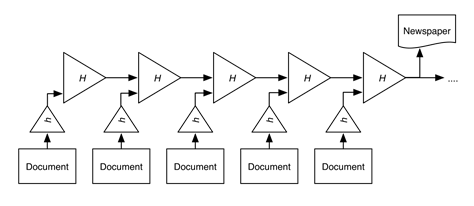
\includegraphics[width=0.7\textwidth]{./figs/hash-chain-with-data.png} 

		\caption{Hash chain with data.}		
		\label{fig:hash-chain-data}

	\end{center}	
\end{figure}

This approach, however, does not scale well with the number of documents
being logged. To address this, documents can be aggregated using data
structures like Merkle trees.

\subsubsection{Merkle Trees}\label{merkle-trees}

A Merkle tree, also known as a hash tree, is a binary tree data
structure in which every leaf node is the hash of a block of data, and
every non-leaf node is the hash of the concatenation of its children's
hashes (see \autoref{fig:merkle-tree}). This structure allows for efficient and secure verification of
the contents of large data sets.

\begin{figure}[t]
	%	\vspace{-0.3cm}
	\begin{center}
		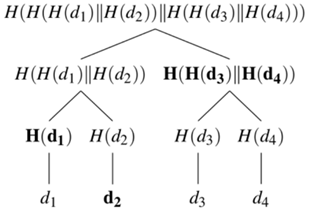
\includegraphics[width=0.5\textwidth]{./figs/merkle-tree.png} 

		\caption{Merkle tree.}		
		\label{fig:merkle-tree}

	\end{center}	
\end{figure}

The construction of a Merkle tree begins at the bottom with the leaf
nodes, which represent the hashes of individual data blocks, such as
transactions in a blockchain. These leaf nodes are then paired, and
their hashes are concatenated and hashed together to form the parent
nodes. This process is repeated recursively until a single root hash is
produced, which is known as the Merkle root.

The Merkle root has the unique property of representing the hash of the
entire data set. Any change to a single data block will result in a
different Merkle root, making it an effective tool for ensuring data
integrity.

One of the most significant advantages of Merkle trees is their ability
to provide \textbf{compact membership proofs}. A membership proof, also
known as an authentication path, allows a user to verify that a specific
piece of data is included in the data set without having to download and
hash the entire set. The proof consists of the leaf hash and the hashes
of the sibling nodes along the path from the leaf to the root. The
verifier can then use this information to reconstruct the Merkle root
and compare it to the known root hash. This process has a logarithmic
time and space complexity, making it highly efficient for large data
sets.

In the context of blockchains, Merkle trees are used to summarize all
the transactions in a block, producing a single Merkle root that is
included in the block header. This allows for efficient verification of
transactions without the need to download the entire block.

\subsubsection{A Combination of Merkle Trees and Hash Chains}\label{a-combination-of-merkle-trees-and-hash-chains}

Data can be aggregated in Merkle trees and added in batches (see \autoref{fig:combination}). The
integrity of the data is represented by the small root hashes, and the
integrity of the whole chain is represented by the last hash in the
chain.

\begin{figure}[t]
	%	\vspace{-0.3cm}
	\begin{center}
		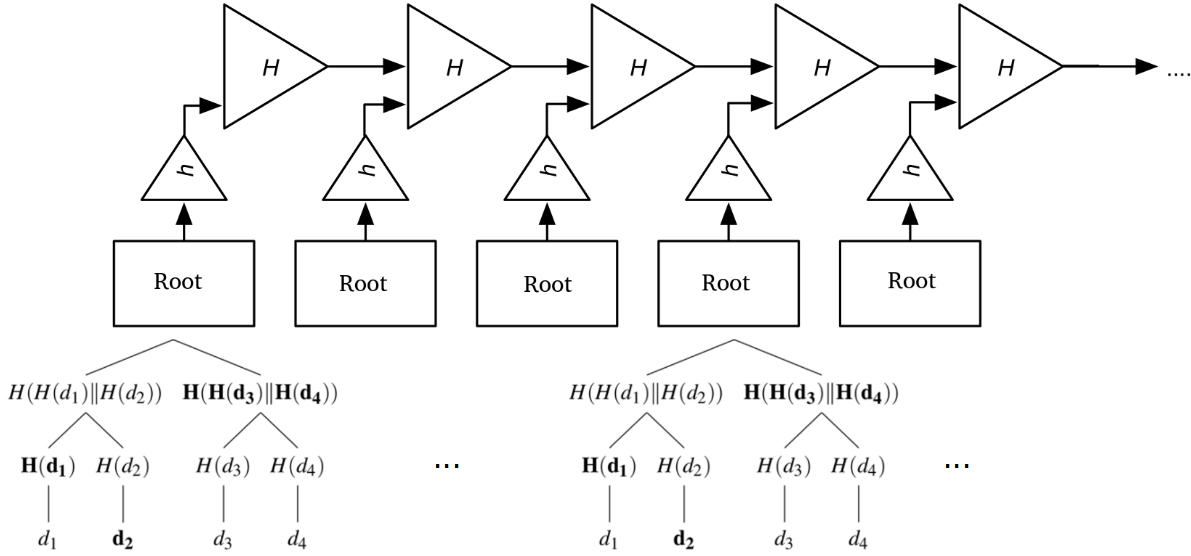
\includegraphics[width=0.9\textwidth]{./figs/combination-mk-hc.png} 

		\caption{A combination of Merkle tree and hash chains.}		
		\label{fig:combination}
	\end{center}	
\end{figure}


\subsubsection{Proof-of-Work (PoW)}\label{proof-of-work-pow}

Proof-of-Work is a mechanism that requires a significant amount of
computational work to be performed in order to achieve a certain goal (see example in \autoref{fig:pow}).
It is a key component of many cryptocurrencies, including Bitcoin.

A non-interactive version of PoW is \textbf{Hashcash}, proposed by Adam
Back in 1997 as a spam prevention mechanism. The idea is that the sender
of an email has to perform some work to send it, making it expensive to
send large volumes of spam. The proof generation is expensive, but the
verification is cheap.

\begin{figure}[!b]
	%	\vspace{-0.3cm}
	\begin{center}
		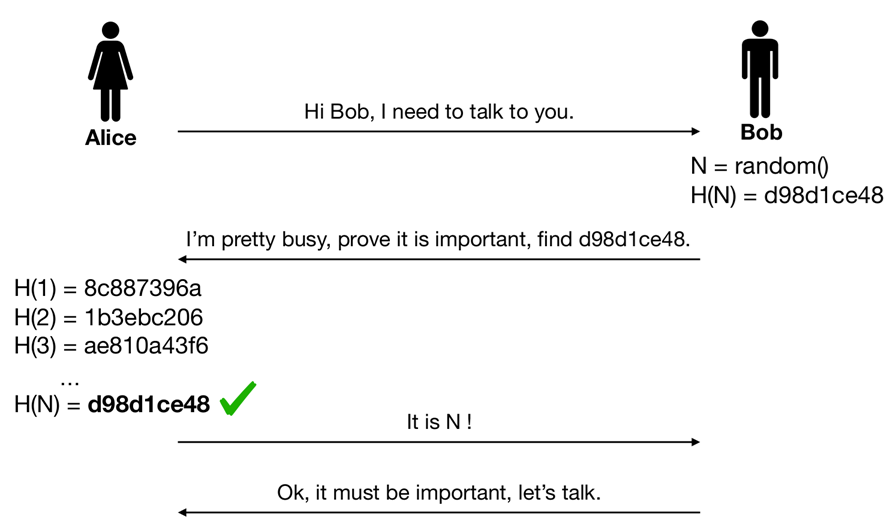
\includegraphics[width=0.8\textwidth]{./figs/pow.png} 
		\caption{Proof-of-Work principle.}		
		\label{fig:pow}
	\end{center}	
\end{figure}


\subsubsection{Commitments}\label{commitments}

A commitment scheme allows one to commit to a chosen value while keeping
it hidden from others, with the ability to reveal the committed value
later.

\begin{itemize}
	\tightlist
	\item
	\textbf{Commit}: Alice picks a value \texttt{x} and sends
	\texttt{H(x)} to Bob. This is the commitment. The use of a hash
	function guarantees the \textbf{binding} property (the commitment is
	bound to \texttt{x}), and since Bob doesn't know \texttt{x}, the
	\textbf{hiding} property is also satisfied.
	\item
	\textbf{Reveal}: Alice reveals \texttt{x} to Bob, who can then verify
	that \texttt{H(x)} matches the commitment he received.
\end{itemize}

\subsubsection{Digital Signatures}\label{digital-signatures}

Digital signatures are a cornerstone of modern cryptography, providing a
means to ensure the authenticity, integrity, and non-repudiation of
digital messages. They are the digital equivalent of a handwritten
signature, but with far stronger security guarantees. Digital signatures
are based on public-key cryptography, which involves a pair of
mathematically related keys: a private key, which is kept secret by the
owner, and a public key, which can be freely distributed.

The fundamental operations of a digital signature scheme are as follows:

\begin{itemize}
	\tightlist
	\item
	\textbf{Key Generation}: A user generates a key pair, consisting of a
	private key (SK) and a corresponding public key (PK).
	\item
	\textbf{Signing}: To sign a message, the user applies a signing
	algorithm to the message and their private key. This produces a
	digital signature, which is a fixed-size string of data (see \autoref{fig:signatures}.
	\item
	\textbf{Verification}: To verify a signature, a recipient uses the
	sender's public key, the message, and the signature. The verification
	algorithm returns a boolean value indicating whether the signature is
	valid (see \autoref{fig:signatures}.
\end{itemize}

\begin{figure}[t]
	%	\vspace{-0.3cm}
	\begin{center}
		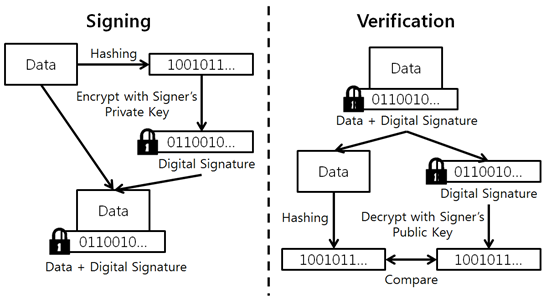
\includegraphics[width=0.7\textwidth]{./figs/signatures.png} 
		\caption{Digital signatures.}		
		\label{fig:signatures}
	\end{center}	
\end{figure}

Digital signatures provide several crucial security properties:

\begin{itemize}
	\tightlist
	\item
	\textbf{Authenticity}: A valid signature confirms that the message was
	signed by the owner of the corresponding private key. This is because
	only the owner of the private key could have produced a valid
	signature that can be verified with the public key.
	\item
	\textbf{Integrity}: The signature ensures that the message has not
	been altered since it was signed. Any modification to the message
	would result in an invalid signature.
	\item
	\textbf{Non-Repudiation}: The signer cannot plausibly deny having
	signed the message, as only they have access to the private key.
	However, it is important to note that this property can be challenged
	if the signer can plausibly claim that their private key was
	compromised.
	\item
	\textbf{Unforgeability}: It is computationally infeasible for an
	attacker to forge a valid signature for a new message without access
	to the private key. This property is based on the computational
	difficulty of the underlying mathematical problems, such as the
	discrete logarithm problem or the integer factorization problem.
\end{itemize}

In the context of blockchains, digital signatures are used to authorize
transactions. When a user wants to send cryptocurrency or interact with
a smart contract, they sign the transaction with their private key. This
signature proves that they are the legitimate owner of the funds or
assets being transferred and that they have authorized the transaction.

\begin{center}\rule{0.5\linewidth}{0.5pt}\end{center}

\subsection{Introduction to
	Blockchains}\label{section-3-introduction-to-blockchains}

\subsubsection{Why Blockchains?}\label{why-blockchains}

The advent of blockchain technology was driven by the inherent
limitations of traditional centralized information systems. These
systems, while ubiquitous, suffer from a number of vulnerabilities that
can compromise their security, reliability, and trustworthiness.

\begin{itemize}
	\tightlist
	\item
	\textbf{Single Point of Failure}: Centralized systems are susceptible
	to a single point of failure. A hardware malfunction, a software bug,
	or a successful denial-of-service (DDoS) attack on a central server
	can render the entire system inoperable.
	\item
	\textbf{Censorship}: A central authority has the power to censor users
	or transactions at its discretion, often without any mechanism for
	appeal or recourse. This can lead to arbitrary exclusion and a lack of
	fairness.
	\item
	\textbf{Limited Availability}: While cloud service providers often
	advertise high availability, achieving 100\% uptime is practically
	impossible in a centralized architecture. Outages can and do occur,
	leading to service disruptions.
	\item
	\textbf{Lack of Data Integrity}: In a centralized database, a
	malicious actor with sufficient privileges can alter or delete data
	without leaving a trace. This makes it difficult to guarantee the
	integrity and authenticity of the data.
	\item
	\textbf{Lack of Transparency}: The inner workings of centralized
	systems are often opaque to users. There is no way to independently
	verify that the system is operating as intended or that the data is
	being handled correctly.
\end{itemize}

Blockchain technology offers a paradigm shift, providing a decentralized
alternative that addresses these challenges through its inherent
properties:

\begin{itemize}
	\tightlist
	\item
	\textbf{Decentralization}: By distributing the ledger across a network
	of nodes, blockchains eliminate the single point of failure. The
	system can continue to operate even if some nodes go offline.
	\item
	\textbf{Censorship Resistance}: In a permissionless blockchain, all
	valid transactions are eventually processed. No single entity has the
	power to censor transactions, ensuring that the network remains open
	and accessible to all.
	\item
	\textbf{Immutability}: The append-only nature of the blockchain,
	enforced by cryptographic hashes, makes it extremely difficult to
	alter or delete past transactions. This creates a permanent and
	tamper-evident record of all activity on the network.
	\item
	\textbf{Auditability}: The entire history of the blockchain is
	available for anyone to inspect and verify. This allows for
	independent auditing of the system, ensuring that all transactions are
	valid and that the rules of the protocol have been followed.
	\item
	\textbf{Transparency}: All transactions on a public blockchain are
	visible to all participants. This transparency fosters trust and
	accountability, as all actions are open to scrutiny.
\end{itemize}

\subsubsection{3.2: High-Level View of
	Blockchains}\label{high-level-view-of-blockchains}

From a high-level perspective, a blockchain can be understood as a
synthesis of three distinct fields:

\begin{figure}[t]
	%	\vspace{-0.3cm}
	\begin{center}
		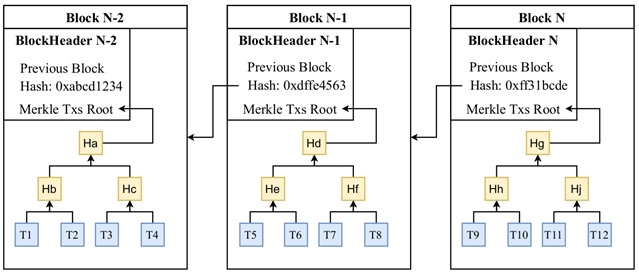
\includegraphics[width=0.8\textwidth]{./figs/blockchain-overview.png} 
		\caption{Overview of blockchain structure.}		
		\label{fig:overview-blockchain}
	\end{center}	
\end{figure}

\begin{itemize}
	\tightlist
	\item
	\textbf{Cryptography}: This provides the fundamental tools for
	securing the data and computations on the blockchain. As discussed in
	the previous section, cryptographic primitives such as hash functions
	and digital signatures are essential for ensuring the integrity,
	authenticity, and immutability of the ledger.
	\item
	\textbf{Distributed Systems}: This field provides the theoretical and
	practical foundations for building and maintaining a decentralized
	network. Blockchains are inherently distributed systems, and they rely
	on concepts from this field to address challenges such as fault
	tolerance, concurrency, and consensus.
	\item
	\textbf{Economics and Game Theory}: This provides the framework for
	designing protocols that incentivize rational actors to behave in a
	manner that is beneficial to the network as a whole. By carefully
	designing the economic incentives, it is possible to create a system
	that is robust and secure, even in the presence of self-interested or
	malicious participants.
\end{itemize}

At its core, a blockchain is a globally shared, append-only database, or
ledger, that is replicated across all participating nodes in the
network. The ledger is modified through the submission of transactions,
which are cryptographically signed by the participants. These
transactions are then bundled together into blocks, which are added to
the chain in a chronological and immutable manner. Each block is linked
to its predecessor by including the hash of the previous block's header,
creating a cryptographically secure chain of blocks that is resistant to
tampering (see \autoref{fig:overview-blockchain}).




\subsubsection{Participants in a Blockchain
	Network}\label{sec:participants-in-a-blockchain-network}

A blockchain network is a diverse ecosystem of participants, each with a
distinct role and level of engagement. The network can be conceptualized
as an inclusive hierarchy, with different types of nodes contributing to
the overall operation and security of the system (see \autoref{fig:participants}).

\begin{figure}[t]
	%	\vspace{-0.3cm}
	\begin{center}
		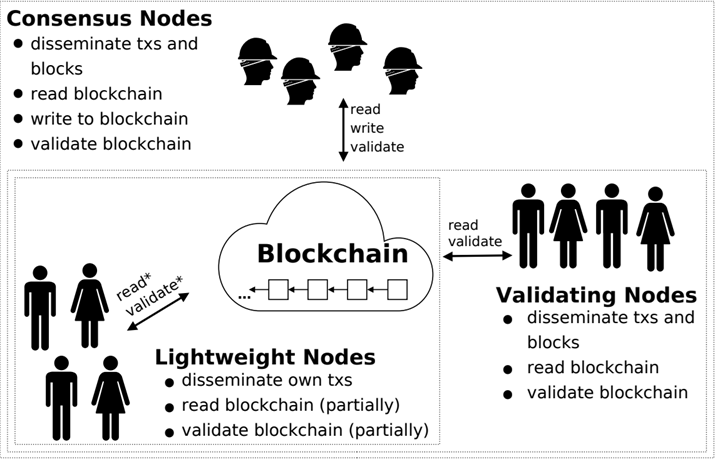
\includegraphics[width=0.8\textwidth]{./figs/participants.png} 
		\caption{Participants in blockchains.}		
		\label{fig:participants}
	\end{center}	
\end{figure}


\begin{itemize}
	\item
	\textbf{Consensus Nodes (Miners/Validators)}: At the top of the
	hierarchy are the consensus nodes, also known as miners in
	Proof-of-Work (PoW) systems or validators in Proof-of-Stake (PoS)
	systems. These nodes are the most active participants in the network,
	and they are responsible for the critical task of creating new blocks.
	This involves collecting and validating transactions, ordering them
	into a new block, and proposing the block to the rest of the network.
	In return for their efforts, consensus nodes are rewarded with newly
	created cryptocurrency and transaction fees.
	\item
	\textbf{Validating Nodes (Full Nodes)}: These nodes form the backbone
	of the network, providing a high level of security and
	decentralization. They download and store a complete copy of the
	blockchain, and they independently validate every transaction and
	block against the protocol's consensus rules. By doing so, they ensure
	that all participants are adhering to the same set of rules and that
	no invalid transactions are included in the ledger. Validating nodes
	also play a crucial role in disseminating transactions and blocks
	throughout the network.
	\item
	\textbf{Lightweight Nodes (Clients)}: These are the most common type
	of node, and they are typically used by end-users to interact with the
	blockchain. Lightweight nodes, as their name suggests, do not store
	the entire blockchain. Instead, they only download and store the block
	headers, which contain a summary of the block's contents, including
	the Merkle root. To verify a transaction, a lightweight node can
	request a membership proof from a full node, which allows it to
	confirm that the transaction is included in a block without having to
	download the entire block. This makes lightweight nodes ideal for use
	on devices with limited storage and bandwidth, such as mobile phones.
\end{itemize}

\subsubsection{How Participants
	Communicate}\label{how-participants-communicate}

Participants in a blockchain network communicate through a peer-to-peer
(P2P) network over-layed over underlying network using a gossiping protocol (see \autoref{fig:network-overlay}). Messages are sent only to a
small number of peers (e.g., 8-50). When a new node joins the network,
it scans a list of hard-coded directory nodes (DNS seeders) to find
peers.

The network propagation delay is a crucial factor. A 2013 study on
Bitcoin showed that the mean time for a block to be seen by 95\% of the
nodes was 12.6 seconds, with a maximum of 40 seconds \ih{cite}.

\begin{figure}[t]
	%	\vspace{-0.3cm}
	\begin{center}
		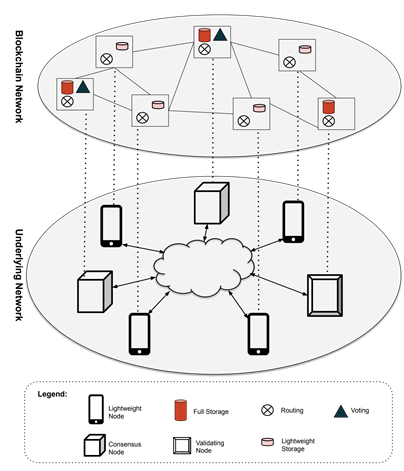
\includegraphics[width=0.4\textwidth]{./figs/network-overlay.png} 
		\caption{Overview of network in blockchains.}		
		\label{fig:network-overlay}
	\end{center}	
\end{figure}

\begin{center}\rule{0.5\linewidth}{0.5pt}\end{center}

\subsection{Summary / Key Takeaways}\label{summary-key-takeaways}

This section has provided a short introduction to the BDA
course, outlining its objectives, structure, and the expertise of its
instructors. It has underscored the critical importance of a strong
technical foundation in the principles of blockchain and decentralized
applications. The section has delved into the essential cryptographic
constructs that form the bedrock of blockchain technology, including:

\begin{itemize}
	\tightlist
	\item
	\textbf{Cryptographic Hash Functions}: Their properties of pre-image
	resistance, second pre-image resistance, and collision resistance are
	fundamental to the integrity and security of the blockchain.
	\item
	\textbf{Hash Chains}: A simple yet powerful method for creating
	sequences of verifiable data, with applications such as one-time
	passwords.
	\item
	\textbf{Merkle Trees}: An efficient data structure for summarizing and
	verifying the integrity of large sets of data, enabling compact
	membership proofs.
	\item
	\textbf{Digital Signatures}: The mechanism for providing authenticity,
	integrity, and non-repudiation in a decentralized environment.
\end{itemize}

The section concluded with a high-level overview of blockchain
technology, highlighting its key features and the problems it aims to
solve. It also provided a classification of the different participants
in a blockchain network, from lightweight clients to consensus nodes.

\begin{center}\rule{0.5\linewidth}{0.5pt}\end{center}

\subsection{Keywords}\label{keywords}

\begin{itemize}
	\tightlist
	\item
	\textbf{Blockchain}: A decentralized, distributed, and immutable
	digital ledger that is used to record transactions across many
	computers so that any involved record cannot be altered retroactively,
	without the alteration of all subsequent blocks.
	\item
	\textbf{Decentralized Application (DApp)}: An application that is run
	by many users on a decentralized network with trustless protocols.
	They are designed to avoid any single point of failure.
	\item
	\textbf{Cryptographic Hash Function}: A mathematical algorithm that
	maps data of arbitrary size to a bit string of a fixed size (a hash)
	and is a one-way function, that is, a function which is practically
	infeasible to invert.
	\item
	\textbf{Merkle Tree}: A tree in which every leaf node is labelled with
	the cryptographic hash of a data block, and every non-leaf node is
	labelled with the cryptographic hash of the labels of its child nodes.
	\item
	\textbf{Digital Signature}: A mathematical scheme for demonstrating
	the authenticity of digital messages or documents. A valid digital
	signature gives a recipient very strong reason to believe that the
	message was created by a known sender (authentication), that the
	sender cannot deny having sent the message (non-repudiation), and that
	the message was not altered in transit (integrity).
	\item
	\textbf{Consensus Protocol}: A set of rules and procedures that allows
	a distributed network of computers to work together to achieve a
	common goal. In the context of blockchains, the consensus protocol is
	what allows the network to agree on the state of the ledger.
	\item
	\textbf{Attacker Model}: A formal model of the capabilities of an
	attacker, used to analyze the security of a system.
	\item
	\textbf{Proof-of-Work (PoW)}: A consensus mechanism that requires a
	significant amount of computational work to be performed in order to
	create a new block.
	\item
	\textbf{Proof-of-Stake (PoS)}: A consensus mechanism in which the
	creator of the next block is chosen in a deterministic way, depending
	on its wealth, also defined as stake.
\end{itemize}

\begin{center}\rule{0.5\linewidth}{0.5pt}\end{center}

\subsection{Further Reading}\label{further-reading}

\begin{itemize}
	\tightlist
	\item
	\textbf{Bitcoin and Cryptocurrency Technologies}:\\
	\url{http://bitcoinbook.cs.princeton.edu/}
	\item
	\textbf{Security Reference Architecture for Blockchains}:\\
	\url{https://ieeexplore.ieee.org/document/9239372}
	\item
	\textbf{Blockchain Technology Course by P. Szalachowski}:\\
	\url{https://github.com/pszal/teaching/tree/master/Blockchain-Technology}
\end{itemize}